\documentclass{standalone}
\usepackage{mathpazo}
\usepackage[american voltages, american currents]{circuitikz}

\begin{document}
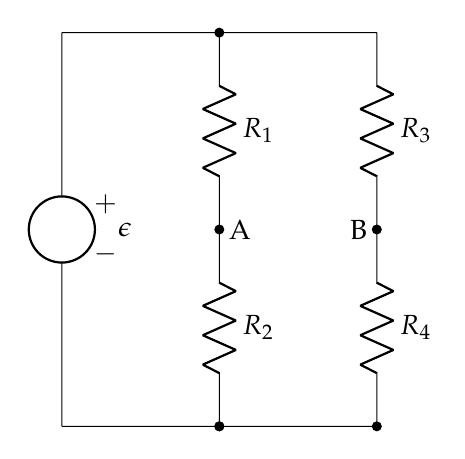
\begin{tikzpicture}
  \coordinate (A) at (0,5);
  \coordinate (B) at (2,5);
  \coordinate (C) at (4,5);
  \coordinate (D) at (0,0);
  \coordinate (E) at (2,0);
  \coordinate (F) at (4,0);
  \draw
  (A) to [short, -*] (B) to [short] (C)
  (D) to [short, -*] (E) to [short] (F)
  (A) to [esource, v = $\epsilon$] (D)
  (B) to [R, l=$R_1$, -*] ++(0,-2.5) node[right] {A}
  to [R, l=$R_2$, -*] (E)
  (C) to [R, l=$R_3$, -*] ++(0,-2.5) node[left] {B}
  to [R, l=$R_4$, -*] (F);
\end{tikzpicture}
\end{document}